

%
% Chapter 5
%

\chapter{SPECTRUM ANALYSIS}
\label{chap:spectrumAnalysis}

Spectrum analysis is a key component of our cooperative strategy. This chapter will discuss the spectrum sensing techniques. Based on the characteristics of the USRP, a new spectrum sensing algorithm is proposed.

\section{Spectrum Sensing}
\label{SpectrumSensingIntro}
The three major types of spectrum sensing techniques include matched filter detection, feature detection, and energy detection \cite{HanoWangGosanNohDongkyuKimSungtaeKimandDaesikHong2010}. In this section, only one frequency band is taken into consideration.

\subsection{Matched Filter Detection}
In digital communication, the matched filter is often used by the receiver to demodulate the digital information from the received waveform \cite{JGProakisMasoudSalehi}. If the primary user's signal is known to the secondary user, the matched filter can also be used to detect whether the primary user is using the spectrum. It is widely known that detection using a matched filter can achieve the optimum performance in white Gaussian noise when a secondary sensing node can perform a coherent detection of the primary user's signal \cite{DCabricandSMMishraandRWBrodersen2004}. With matched filter based sensing, it takes less time to achieve a limited probability of a missed detection and a false alarm. The required number of samples is inversely proportional to the SNR for a given confidence level of a false alarm \cite{R.TandraandA.Sahai:2005}. The main defect for matched filter detection is that the sensing node must have prior knowledge of other radios such as the preamble signaling for synchronization, modulation scheme, etc., which may not be possible.

\subsection{Feature Detection}
The feature detection method utilizes some features of the radios using this spectrum band. Since no prior knowledge is known in the Spectrum Challenge, this technique cannot be used, but we still briefly introduce it.

\subsubsection{Waveform Based Sensing}
In waveform based sensing, the sensing node needs to know the patterns of the other radios, such as preambles, pilots, and spreading sequences. Sensing can be performed by correlating the received signal with known signals \cite{A.SahaiandR.TandraandS.M.MishraandN.Hoven:2006}. The difference between matched filter detection and waveform based sensing is that matched filter detection requires perfect modulation information of primary users while the waveform based sensing only needs some signal patterns of the primary users.

\subsubsection{Cyclostationarity-Based Sensing}
Cyclostationary features can be used for spectrum sensing. Usually cyclostationary features are inherent in the signal's statistics, such as mean and autocorrelation, or through the signal's periodicity. In addition, cyclostationary can be introduced into the primary users' signal to aid spectrum detection. Some OFDM systems have been altered to adapt to the requirements of cyclostationarity-based sensing \cite{P.D.SuttonandK.E.NolanandL.E.Doyle:2007}. Since noise is often modeled as wide-sense stationary (WSS), cyclostationarity-based detection can more easily distinguish between the users' signal and noise.

\subsubsection{Radio Identification Based Sensing}
Knowledge about the spectrum characteristics can be obtained by learning the transmission technologies of transmitting users, and such characteristics can be used to help characterize spectrum usage. For instance, suppose one radio can be identified as employing WiFi signals. The sensing node can use this information to conclude that the radio should be within 100 meters. In radio identification based sensing, several features can be used to determine the transmission technologies. These features include amount of the energy detected and the energy distribution across the spectrum, channel bandwidth and the shape signal \cite{J.PalicotandC.Roland:2003}. These features are fed to a Bayesian classifier for determining the active radios.

\subsection{Energy Detection}
Energy detection is the most common spectrum sensing technique. It has low implementation and computational complexities \cite{M.Wylie-Green:2005}. Receivers that use energy detection do not need detailed knowledge of the modulation schemes of the primary users. They only need to detect whether the signal level exceeds a certain threshold determined by the noise level. Assume $s(n)$ is the primary uses' signal, $w(n)$ is additive white Gaussian noise (AWGN) and $y(n)$ is the received signal of the secondary user. The system model is
\begin{align}
y(n)=s(n)+w(n).
\label{systemModel}
\end{align}
Making a decision whether primary users are using the spectrum is equivalent to the following hypotheses:
\begin{align}
&\mathcal{H}_0:y(n)=w(n)\\
&\mathcal{H}_1:y(n)=s(n)+w(n).
\end{align}
Here $\mathcal{H}_0$ is the null hypothesis that the primary users are not using the spectrum, while $\mathcal{H}_1$ is the hypothesis that the primary users are using the spectrum.

The decision statistic based upon received energy is
\begin{align}
E=\frac{1}{N}{\sum\limits_{n = 1}^N {\left| {y(n)} \right|} ^2}.
\label{decisionMetricTime}
\end{align}
Define the probability of detection to be $P_D$, the probability of false alarm to be $P_F$, and the probability of missed detection to be $P_M$. Then
\begin{align}
&P_D=P_r(E > \lambda_E | \mathcal{H}_1)
\label{Detectionprobability}\\
&P_F=P_r(E > \lambda_E | \mathcal{H}_0)\\
&P_M=P_r(E \leq \lambda_E | \mathcal{H}_1)=1-P_D,
\end{align}
where $\lambda_E$ is the detection threshold of energy detection.  The threshold $\lambda_E$ should be selected such that both $P_F$ and $P_M$ are as small as possible. However, a tradeoff exists between $P_F$ and $P_M$.  The threshold $\lambda_E$ depends on the noise variance, and even a small estimation error of noise variance would cause a significance detection error \cite{A.SahaiandN.HovenandR.Tandra:2004}. To solve this problem, the noise level can be estimated by separating the signal subspaces and noise dynamically with the multiple signal classification (MUSIC) algorithm \cite{M.P.OlivieriandG.BarnettandA.LackpourandA.Davis:2005}.

\section{Design and Implementation of a Spectrum Analyzer}
From the discussion of Section \ref{SpectrumSensingIntro}, only energy detection does not requires prior knowledge of the characteristics of other radios. As a result, energy detection will be used in our spectrum analyzer.

From Chapter \ref{chap:strategy}, our cooperative radio tries to occupy the entire spectrum left by others. To fulfill this requirement, the 5 MHz bandwidth is divided into 16 sub-bands, and each sub-band can be setup to be used or not based upon energy detection in each sub-band. The data transmitted by each sub-band should not depend on the success of other sub-bands. Define the data transmitted by each sub-band as a physical-layer packet. This process can be viewed as quantization of frequency. Even if only part of the sub-band is used by other radios, it should be marked as used. Therefore, decreasing the bandwidth of each sub-band gives us more spectrum opportunities. In practice, a physical-layer packet should have header information to tell what is included. The length in time of each sub-band has been fixed by the physical layer. If the bandwidth of a sub-band is too small, most of the information carried by a physical-layer packet is header information. Only a small amount of data is transmitted, and the total efficiency decreases. As discussed in Chapter \ref{chap:backgound}, the number of sub-bands for both data transmission is 16, and the number of sub-band for spectrum sensing is also selected to be 16 such that the tone assignment for each sub-band is the same for both data transmission and spectrum sensing.


Figure \ref{fig:SpectrumAnalyzerFlowChart} shows the flow chart of the spectrum analyzer. The software component of the analyzer consists of preprocessing and decision making.

\begin{figure}[tpb]
  \begin{center}
    \centerline{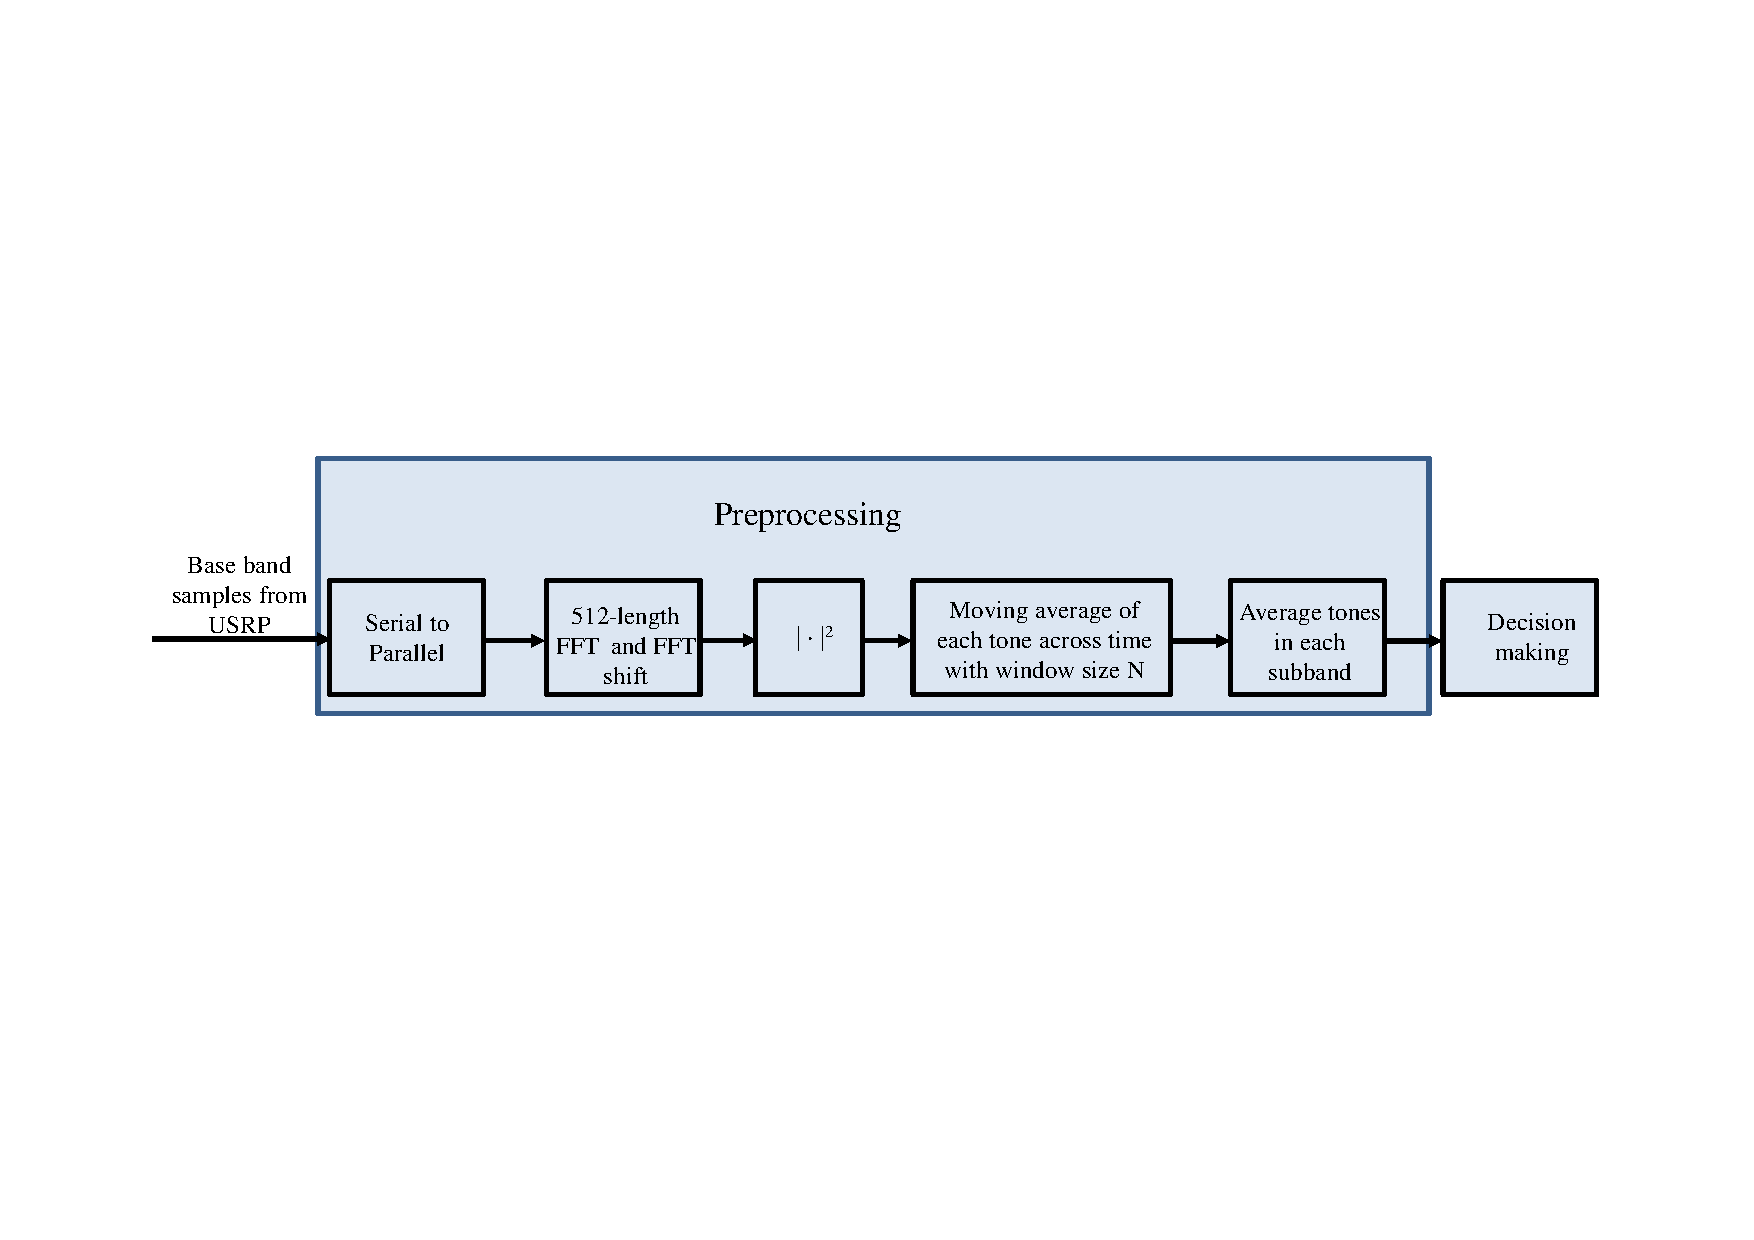
\includegraphics[width=160mm]{SpectrumAnalyzerFlowChart.pdf}}
    \caption{Flow Chart of Spectrum Analyzer}
    \label{fig:SpectrumAnalyzerFlowChart}
  \end{center}
\end{figure}

\subsection{Preprocessing}
First, the serial samples from the USRP are converted to parallel signal with length 512. Second, a length 512 FFT is conducted to convert the signal from the time-domain to the frequency-domain. An FFT shift is conducted to convert the signal from $\left[ {0,2\pi } \right)$ to $\left[ { - \pi ,\pi } \right)$ such that the DC tone is in the center and has index 257. Third, the energy of each frequency sample is calculated. Fourth, the moving average of each tone across time is computed as
\begin{align}
{E_j} = \frac{1}{N}\sum\limits_{n = 1}^N {{{\left| {{s_j}(n)} \right|}^2}}, \quad j = 1,2,...,512,
\label{decisionMetricfreq}
\end{align}
where ${s_j}(n)$ is the signal of tone $j$ at time $n$. Equation (\ref{decisionMetricfreq}) is a modified version of (\ref{decisionMetricTime}). Fifth, the tones in each sub-band are averaged according to
\begin{align}
{E_i} = \frac{1}{M}\sum\limits_{j \in {\rm{sub\mbox{-}band}} \ i}^{} {{E_j}} , \quad i = 1,2,...,16,
\label{subbandEnergy}
\end{align}
where $M$ is the number of tones in each sub-band. Here we have $M=30$.

The feedback of the cooperative radio is sent with a 200 kHz OFDM signal, and the center frequency of the feedback is in the middle of the sub-band that has lowest average energy. In other words, the feedback band is within sub-band ${i^*} = \mathop {\arg \min }\limits_{{\rm{i  =  1,2,}}...{\rm{,16}}} \left\{ {{E_i}} \right\}$.


\subsection{Decisions Making}
In energy detection, comparing the energy of a sub-band to a threshold is the way to decide if the sub-band is used by other radios. However, we observed that sometimes the energy detection used in (\ref{Detectionprobability}) is too conservative. For example, there are strong side lobes for the signal generated by the GNU Radio and the USRP as illustrated in Figure \ref{fig:SginalWithSideLobe}, which was generated by a hardware spectrum analyzer. There are three energy levels in the signal. The highest energy level is the information signal that carries data from the cooperator. The second highest energy level is the side lobe of the cooperator's signal. The lowest energy level is the noise floor. The spectrum occupied by the side lobes can still be used to transmit data as long as we are not generating interference for our cooperators.
\begin{figure}[tpb]
  \begin{center}
    \centerline{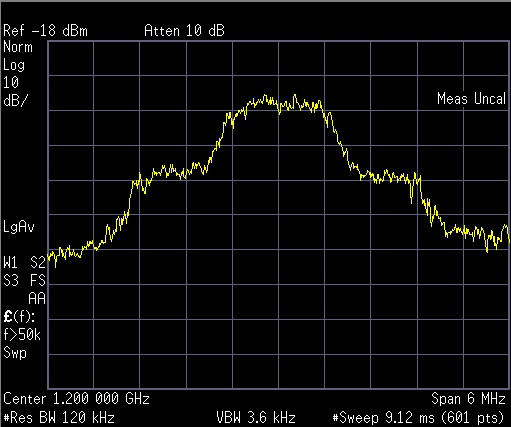
\includegraphics[width=140mm]{SginalWithSideLobe.jpg}}
    \caption{Example of a signal with large side lobes}
    \label{fig:SginalWithSideLobe}
  \end{center}
\end{figure}

A new algorithm is proposed to address the conservative nature of energy detection in the case of strong side lobes. The assumption of the algorithm is that the side lobes are much smaller than main lobe. If the energy level of the side lobes is equivalent to that of the information signal, we cannot distinguish them.

\subsubsection{Signal Model}
As shown in Figure \ref{fig:SpectrumAnalyzerModel}, there are a total of $K=16$ sub-bands, and sub-band $i$ has energy $E_i$ as described in (\ref{subbandEnergy}).We classify signals as the information signal, the side lobe, and the noise. Suppose the information signal energy has mean $m_1$ , and the side lobe energy has mean $m_2$.
\begin{figure}[tpb]
  \begin{center}
    \centerline{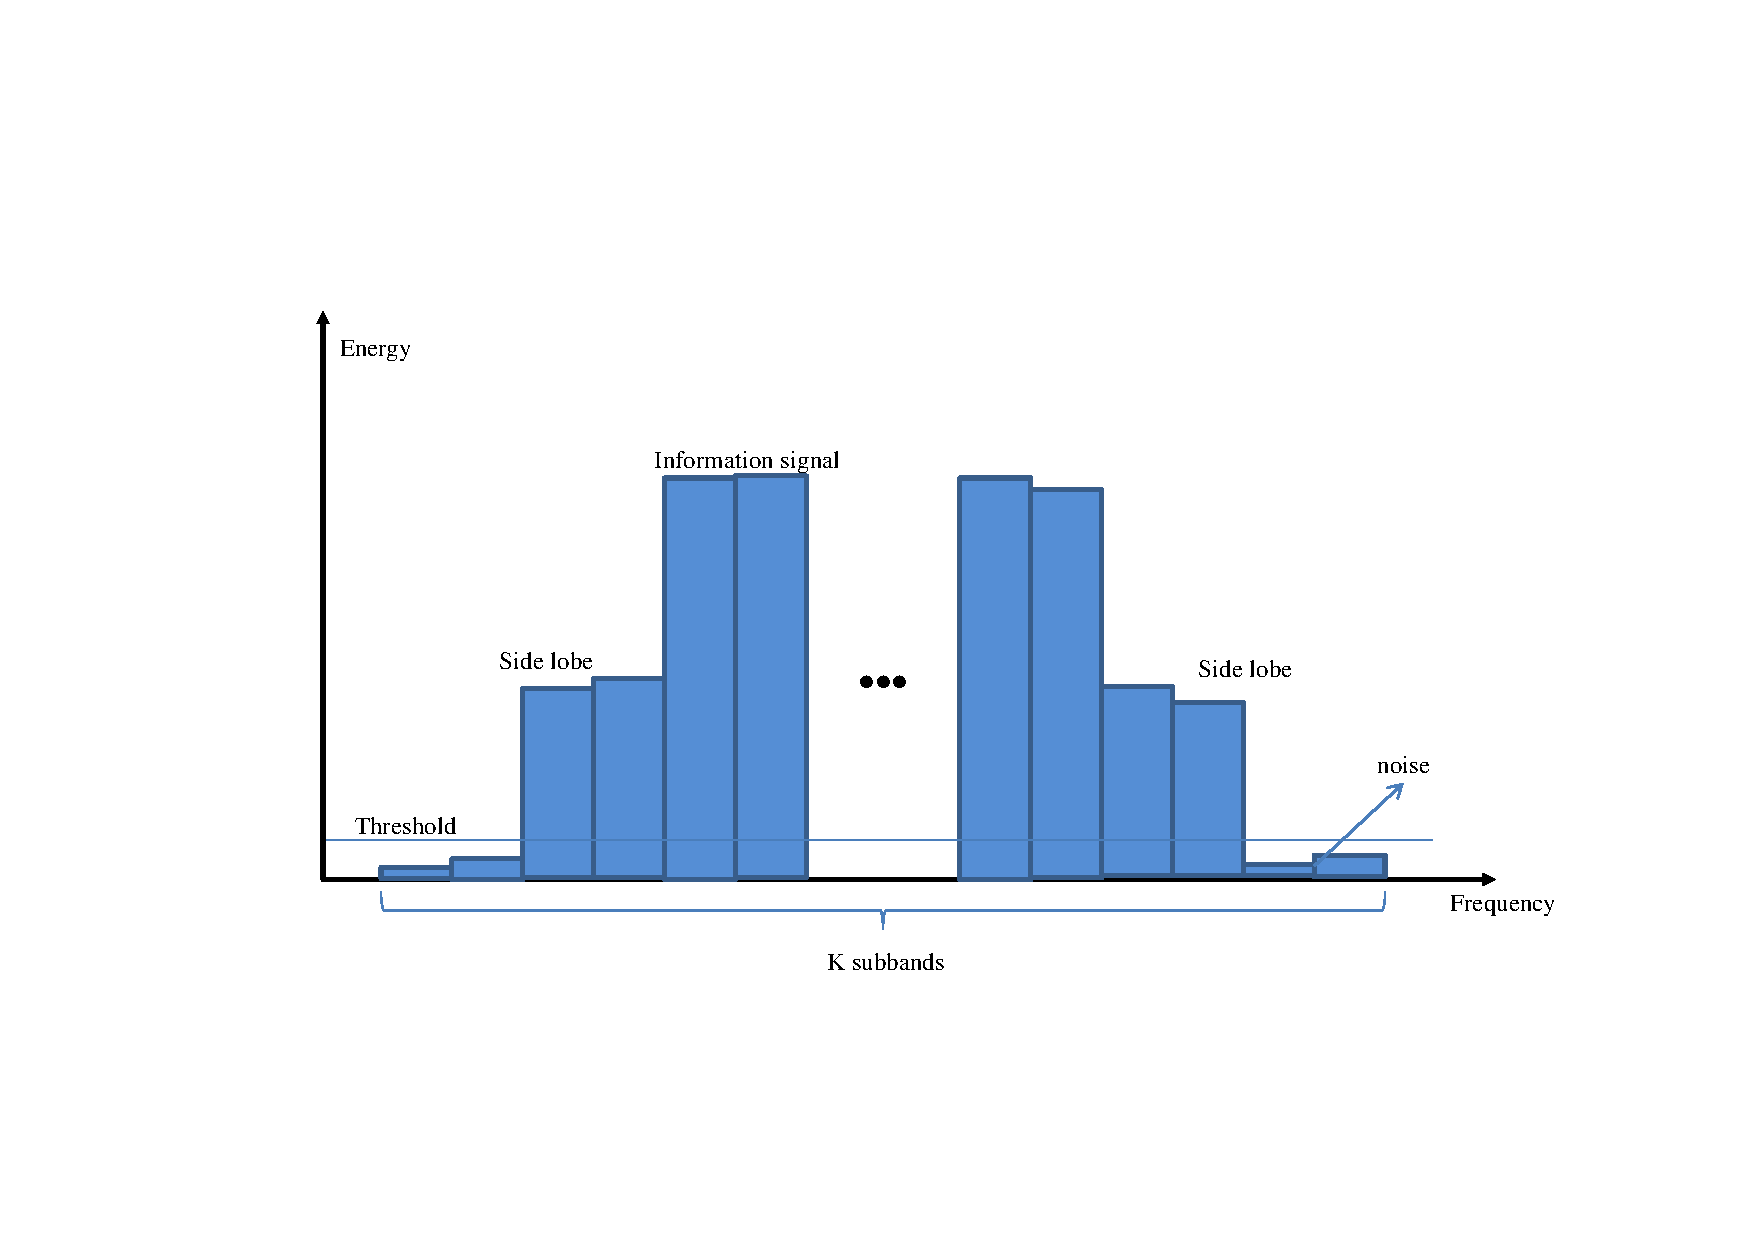
\includegraphics[width=140mm]{SpectrumAnalyzerModel.pdf}}
    \caption{Model illustration of spectrum analyzer}
    \label{fig:SpectrumAnalyzerModel}
  \end{center}
\end{figure}
\subsubsection{Decision Procedures}
First, compare $E_i$ with a threshold $\lambda>0$. If
\begin{align}
E_i < \lambda,
\end{align}
sub-band $i$ is available for use.

Second, consider all the sub-bands for which $E_i  \ge \lambda$. Define
\begin{align}
\mathcal{R}_0 =\left\{ {i:{E_i} \ge \lambda } \right\}.
\end{align}
Suppose the sample mean of their energy is $m_0$ and the sample variance deviation is $S_0^2$, where
\begin{align}
{m_0} = \frac{1}{{\left| \mathcal{R}_0 \right|}}\sum\limits_{i \in \mathcal{R}_0} {{E_i}}
\end{align}
\begin{align}
S_0^2 = \frac{1}{{\left| \mathcal{R}_0 \right| - 1}}\sum\limits_{i \in \mathcal{R}_0} {{{\left( {{E_i} - {m_0}} \right)}^2}}.
\end{align}

If the number of sub-bands in $\mathcal{R}_0 $ is less than 4, we terminate; treating all the remaining sub-bands as a cooperator's signal. The reason for this procedure is that the variance is difficult to estimate from a small sample. Otherwise, if
\begin{align}
\gamma S_0<m_0,
\label{smallvariance}
\end{align}
we treat all the remaining sub-bands as signal from the cooperator and terminate. Here, $\gamma$ is a coefficient to be determined. The reasoning behind (\ref{smallvariance}) is that a small value of $S_0$ indicates that there is not a side lobe, or the side lobes have a similar energy level to the information signal, which cannot be distinguished using energy detection. This step also avoids the situation in which the entire 5 MHz spectrum is occupied by a uniformly distributed signal across frequency.

Finally, for all sub-bands with $E_i \ge \lambda$, if
\begin{align}
E_i \le m_0-\beta S_0,
\label{DecisionCretia}
\end{align}
then sub-band $i$ is available to use, because sub-band $i$ is occupied by a side lobe. Otherwise, sub-band $i$ is considered to be part of the cooperator's information signal.

\subsubsection{Determination of Coefficients $\gamma$ and $\beta$}
The parameter $\gamma$ is used to decide whether there is side lobe. It should be a real number larger than 1, and it is determined by the variance of the cooperator's signal. Two USRPs are used to measure the sample mean to standard deviation ratio. One is used as the spectrum analyzer and the other is used as the interference source. The distance between the two USRPs is about 3 feet. A single-band signal with low-energy side lobes as shown in Figure \ref{fig:SAsingleNoSideLobe} and a single-band signal with large bandwidth as shown in Figure \ref{fig:SASingleLargeBand}, are tested to determine $\gamma$. Twenty tests are conducted. For the information signal, the sample mean to standard deviation ratio in Figure \ref{fig:SAsingleNoSideLobe} is 2.98 on average with a minimum value 2.46; the sample mean to standard deviation ratio in Figure \ref{fig:SASingleLargeBand} is 3.23 on average with a minimum value 2.70. For the information signal plus two side lobes, the sample mean to standard deviation ratio in Figure \ref{fig:SAsingleNoSideLobe} is 1.10 on average with a maximum value 1.29; the sample mean to standard deviation ratio in Figure \ref{fig:SASingleLargeBand} is 1.05 on average with a maximum value 1.16. We choose the value of $\gamma =2$, because 2 is able to distinguish whether there is side lobes form the measurements.

\begin{figure}[tpb]
  \begin{center}
    \centerline{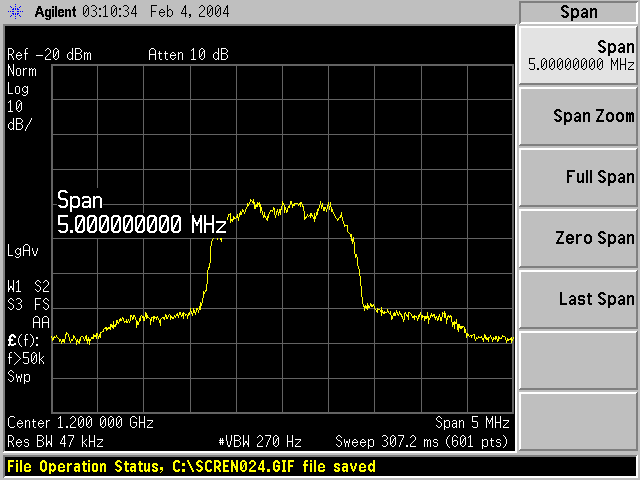
\includegraphics[width=110mm]{SAsingleNoSideLobe.png}}
    \caption{Spectrum of single-band signal with low-energy side lobes. Measured by Agilent E4440A PSA Series Spectrum Analyzer.}
    \label{fig:SAsingleNoSideLobe}
  \end{center}
\end{figure}


\begin{figure}[tpb]
  \begin{center}
    \centerline{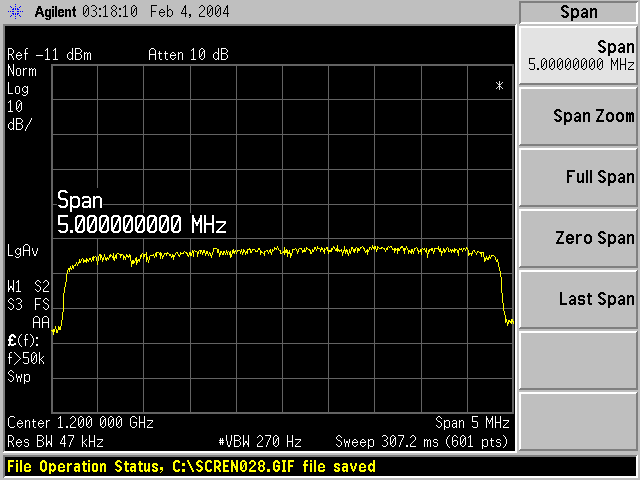
\includegraphics[width=110mm]{SASingleLargeBand.png}}
    \caption{Spectrum of single-band signal with large bandwidth. Measured by Agilent E4440A PSA Series Spectrum Analyzer.}
    \label{fig:SASingleLargeBand}
  \end{center}
\end{figure}


To determine the value of $\beta$, there is an assumption that all sub-bands with the information signal have the same signal level and all sub-bands with the side lobe signal have the same signal level. Suppose the number of sub-bands with information signal is $n_1$, and the number of sub-bands with side lobe is $n_2$. The achievable region of $\left( {{n_1},{n_2}} \right)$ is
\begin{align}
\mathcal{R} =\left\{ {\left( {{n_1},{n_2}} \right):{n_1},{n_2} \in {\mathbb{Z}^ + };{n_1} + {n_2} \le 16} \right\}.
\end{align}
Let
\begin{align}
m_2=\alpha m_1, \quad \alpha<1.
\end{align}
Then
\begin{align}
{m_0} = \frac{{{n_1}{m_1} + {n_2}{m_2}}}{{{n_1} + {n_2}}} = \frac{{{n_1}{m_1} + {n_2}\alpha {m_1}}}{{{n_1} + {n_2}}} = \frac{{{n_1} + {n_2}\alpha }}{{{n_1} + {n_2}}}{m_1}
\end{align}
\begin{align}
{S_0} &= \sqrt {\frac{1}{{{n_1} + {n_2} - 1}}\left[ {{n_1}{{\left( {{m_1} - {m_0}} \right)}^2} + {n_2}{{\left( {{m_2} - {m_0}} \right)}^2}} \right]}&\\
&= \sqrt {\frac{1}{{{n_1} + {n_2} - 1}}\left[ {{n_1}{{\left( {{m_1} - \frac{{{n_1} + {n_2}\alpha }}{{{n_1} + {n_2}}}{m_1}} \right)}^2} + {n_2}{{\left( {\alpha {m_1} - \frac{{{n_1} + {n_2}\alpha }}{{{n_1} + {n_2}}}{m_1}} \right)}^2}} \right]}&\\
&={m_1}\left( {1 - \alpha } \right)\sqrt {\frac{{{n_1}{n_2}}}{{\left( {{n_1} + {n_2} - 1} \right)\left( {{n_1} + {n_2}} \right)}}}.&
\label{S0finalvalue}
\end{align}

From (\ref{DecisionCretia}) and (\ref{S0finalvalue})
\begin{align}
\beta  &\le \frac{{{m_0} - {E_i}}}{{{S_0}}}&\\
&= \frac{{\frac{{{n_1} + {n_2}\alpha }}{{{n_1} + {n_2}}}{m_1} - \alpha {m_1}}}{{{m_1}\left( {1 - \alpha } \right)\sqrt {\frac{{{n_1}{n_2}}}{{\left( {{n_1} + {n_2} - 1} \right)\left( {{n_1} + {n_2}} \right)}}} }}&\\
&= \sqrt {\frac{{{n_1}\left( {{n_1} + {n_2} - 1} \right)}}{{{n_2}\left( {{n_1} + {n_2}} \right)}}}.&
\end{align}
Considering all the possible values of $n_1$ and $n_2$ in the achievable region, we can determine
\begin{align}
\mathop {\min }\limits_{\left( {{n_1},{n_2}} \right) \in {\cal R}} \left\{ {\sqrt {\frac{{{n_1}\left( {{n_1} + {n_2} - 1} \right)}}{{{n_2}\left( {{n_1} + {n_2}} \right)}}} } \right\}=\frac{1}{4}
\end{align}
when $n_1=1$ and $n_2=15$. As a result $\beta \le \frac{1}{4}$ detects all the side lobes based on the criteria of (\ref{DecisionCretia}). A more conservative value of $\beta = \frac{1}{8}$ is chosen for the spectrum analyzer.

\section{Performance of the Spectrum Analyzer}

\subsection{System Setup}
The test setup for assessment of the spectrum analyzer is shown in Figure~\ref{fig:SpectrumAnalyzerSetup}. One USRP is used as a receiver for the spectrum analyzer, and another two USRPs are used as interference sources. The distance between the spectrum analyzer and the interference source is about 3 feet. A Marconi Instruments 2041 low noise signal generator is also used to generate tone interference as shown in Figure \ref{fig:SAsingleTone}
\begin{figure}[tpb]
  \begin{center}
    \centerline{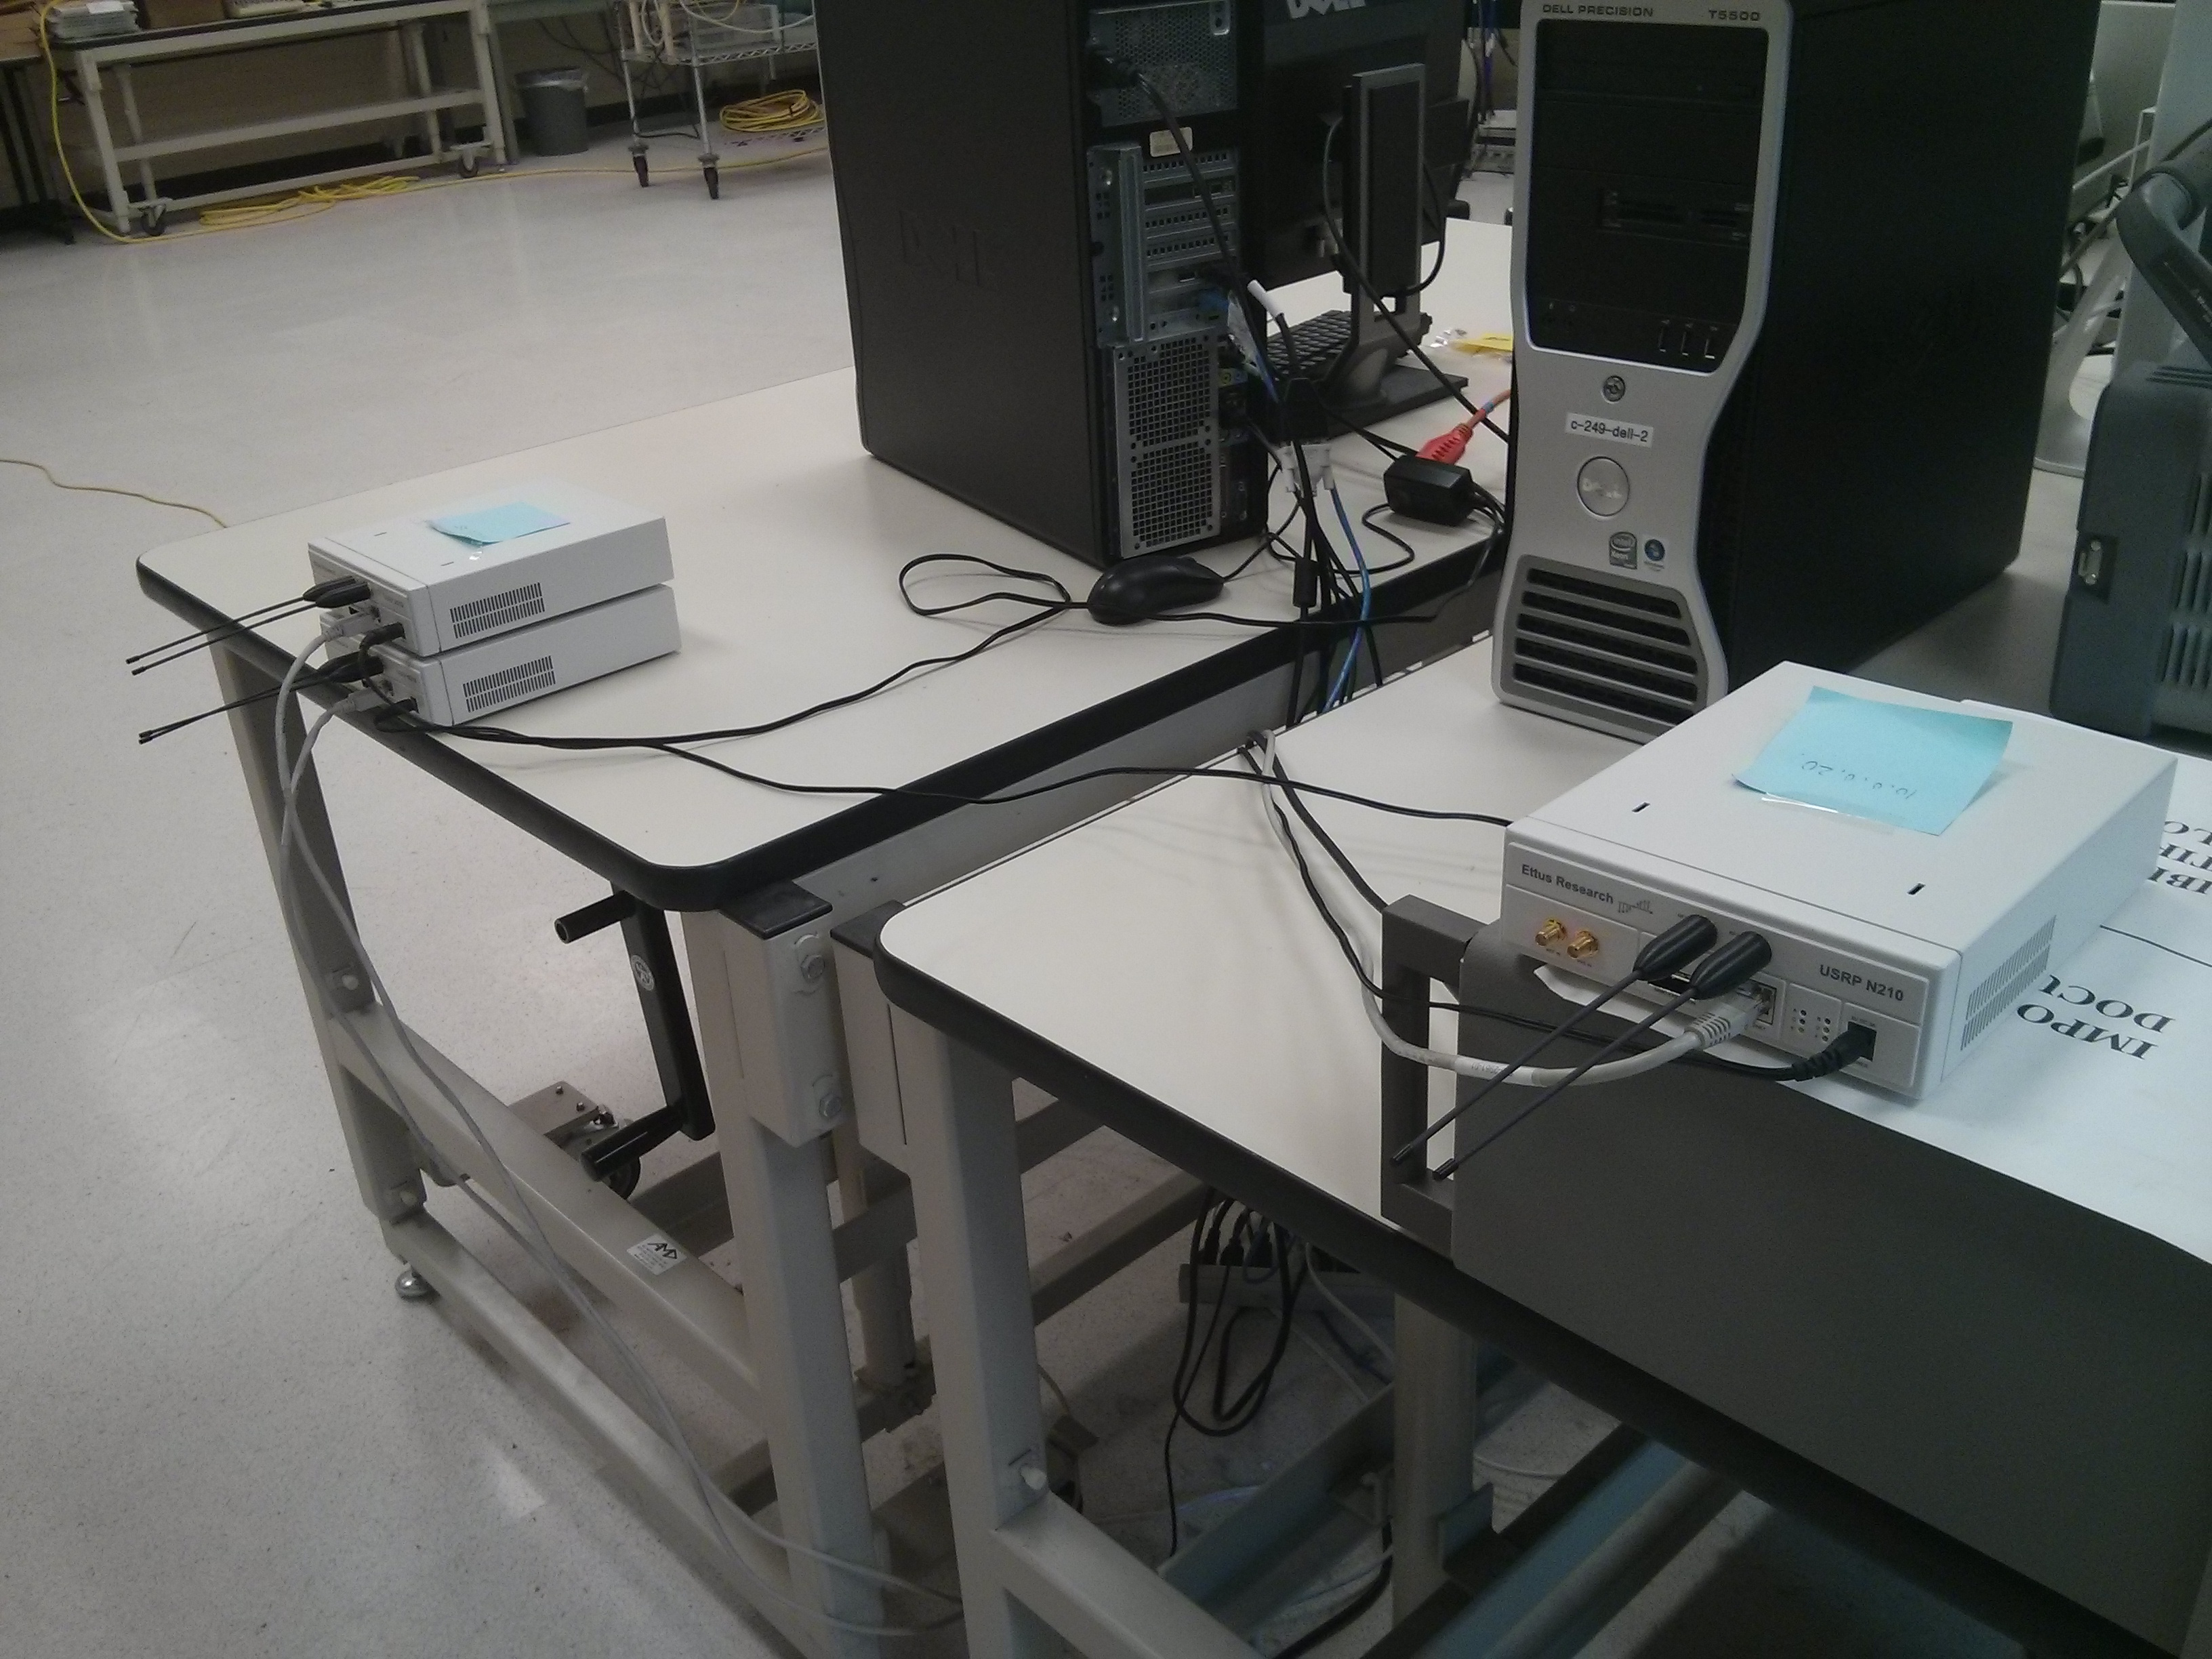
\includegraphics[width=160mm]{SpectrumAnalyzerSetup.jpg}}
    \caption{Setup of spectrum analyzer (right) and interference sources (left). Separation distance is approximately 3 feet.}
    \label{fig:SpectrumAnalyzerSetup}
  \end{center}
\end{figure}

\subsection{Testing Result}
Table \ref{tbl:SAtestResult} lists the detection results of the spectrum analyzer with different types of interference or cooperators' signal, including a sinusoid tone as shown in Figure \ref{fig:SAsingleTone},  a single-carrier signal with side lobes (SSSL) as shown in Figure \ref{fig:SAsinglewithSideLob}, a single-carrier signal with low-energy side lobes (SSLSL) as shown in Figure \ref{fig:SAsingleNoSideLobe}, a single-band signal with large bandwidth (SSLB) as shown in Figure \ref{fig:SASingleLargeBand}, and a two-band signal with side lobes (TSSL) as shown in Figure \ref{fig:SAtwoSignal}. Let 1 denote that a sub-band is available for use and 0 denote the sub-band is our cooperator's signal. The spectrum analyzer is run 1000 times, and the rate of sub-band availability is calculated.

Test results show that the spectrum analyzer can detect the interference and ignore the side lobes. There is small rate of missed detection, such as the sensing results of sub-band 9 and 10 for SSLSL, which is tolerable.

%\begin{table}[tpb]
%  \begin{center}
%    \caption{TEST RESULT��OF SPECTRUM ANALYZER \label{tbl:SAtestResult}}
%    \begin{tabularx}{0.85\textwidth}{llr} \toprule
%      {Test No.}  &  Interference type     &  Availble sub-band  \\ \midrule
%1     &{\begin{tabular}{@{}l@{}} Tone\end{tabular}}                               &1111111011111111 \\\bottomrule
%2     &{\begin{tabular}{@{}l@{}} Single-band signal\\ with side lobes\end{tabular}}           &1111100000011111 \\\bottomrule
%3     &{\begin{tabular}{@{}l@{}} Single-band signal\\ with low-energy side lobes\end{tabular}} &1111100000011111 \\\bottomrule
%4     &{\begin{tabular}{@{}l@{}} Single-band signal\\ with large bandwidth \end{tabular}}      &0000000000000000 \\\bottomrule
%5     &{\begin{tabular}{@{}l@{}} Two-band signal \\with side lobes\end{tabular}}               &1000000110000001 \\ \bottomrule
%    \end{tabularx}
%  \end{center}
%\end{table}

\begin{table}
\centering
    \caption{TEST RESULT: RATE OF SUB-BAND AVAILABILITY (1000 TRAILS) \label{tbl:SAtestResult}}
    \begin{tabular}{cccccc} \toprule
      {Sub-band index}
      &{\begin{tabular}{@{}l@{}} Tone\end{tabular}}
      &{\begin{tabular}{@{}l@{}} SSSL\end{tabular}}
      &{\begin{tabular}{@{}l@{}} SSLSL\end{tabular}}
      &{\begin{tabular}{@{}l@{}} SSLB \end{tabular}}
      &{\begin{tabular}{@{}l@{}} TSSL\end{tabular}}   \\ \bottomrule
1     &1.000    &1.000  &1.000  &0.163  &1.000  \\\bottomrule
2     &1.000    &1.000  &1.000  &0      &1.000  \\\bottomrule
3     &1.000    &1.000  &1.000  &0      &0.984  \\\bottomrule
4     &1.000    &1.000  &1.000  &0      &1.000  \\\bottomrule
5     &1.000    &1.000  &1.000  &0      &0      \\\bottomrule
6     &1.000    &1.000  &1.000  &0      &0      \\\bottomrule
7     &1.000    &0      &0      &0      &0      \\\bottomrule
8     &0        &0      &0      &0      &0      \\\bottomrule
9     &1.000    &0      &0.014  &0      &1.000  \\\bottomrule
10    &1.000    &0      &0.014  &0      &1.000  \\\bottomrule
11    &1.000    &1.000  &1.000  &0      &0      \\\bottomrule
12    &1.000    &1.000  &1.000  &0      &0      \\\bottomrule
13    &1.000    &1.000  &1.000  &0      &0      \\\bottomrule
14    &1.000    &1.000  &1.000  &0      &0.427  \\\bottomrule
15    &1.000    &1.000  &1.000  &0      &1.000  \\\bottomrule
16    &1.000    &1.000  &1.000  &0.361  &1.000  \\\bottomrule
    \end{tabular}
\end{table}



\begin{figure}[tpb]
  \begin{center}
    \centerline{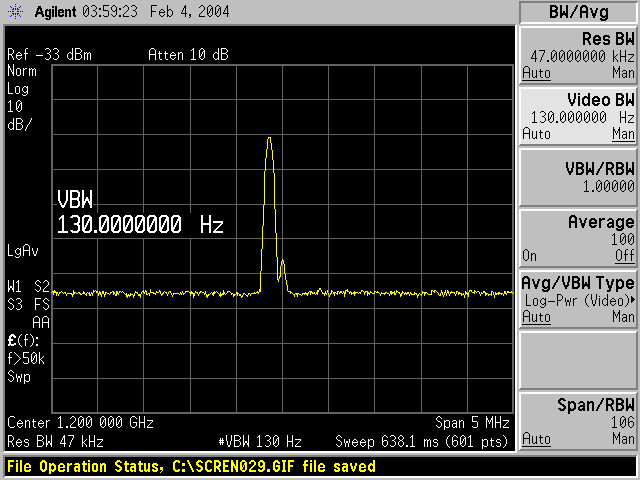
\includegraphics[width=110mm]{SAsingleTone.png}}
    \caption{Spectrum of sinusoid signal. Signal generated by Marconi instruments 2041 low noise signal generator. Measured by Agilent E4440A PSA Series Spectrum Analyzer.}
    \label{fig:SAsingleTone}
  \end{center}
\end{figure}


\begin{figure}[tpb]
  \begin{center}
    \centerline{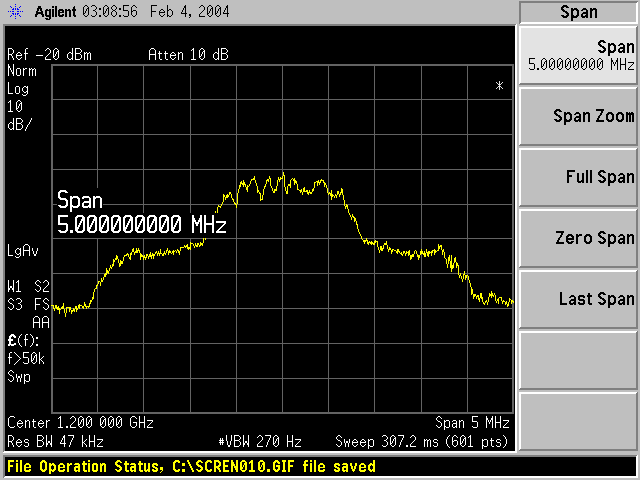
\includegraphics[width=110mm]{SAsinglewithSideLob.png}}
    \caption{Spectrum of single-band signal with side lobes. Measured by Agilent E4440A PSA Series Spectrum Analyzer.}
    \label{fig:SAsinglewithSideLob}
  \end{center}
\end{figure}


\begin{figure}[tpb]
  \begin{center}
    \centerline{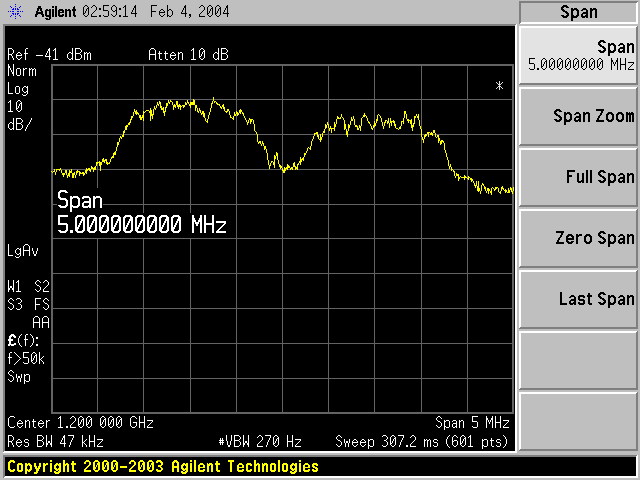
\includegraphics[width=110mm]{SAtwoSignal.png}}
    \caption{Spectrum of two-band signal with side lobes. Measured by Agilent E4440A PSA Series Spectrum Analyzer.}
    \label{fig:SAtwoSignal}
  \end{center}
\end{figure}



